\section{Sessão 2}

Nesta sessão de laboratório, pretende-se estudar alguns componentes de um detetor de proximidade baseado na emissão de infravermelhos (IV), cujo esquema completo está representado na Fig. \ref{fig:park_aid_scheme}. Em \ref{oscilador}, estuda-se o sistema de emissão e, em \ref{filtro_rauch}, simula-se a distância a um obstáculo através de um circuito atenuador e estuda-se um exemplo de um filtro passa-banda que se poderia utilizar para filtrar o sinal obtido à saída do recetor de IV.

\begin{figure}[ht]
    \centering
    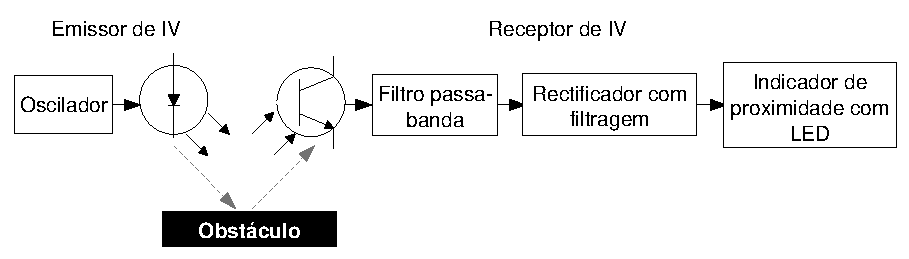
\includegraphics{Imagens/park_aid_scheme.pdf}
    \caption{Esquema completo do detetor de proximidade.}
    \label{fig:park_aid_scheme}
\end{figure}

\subsection{Oscilador de Onda Rectangular} \label{oscilador}

O oscilador de onda retangular permite a emissão do sinal IV ao excitar periodicamente o díodo que o emite. O cirucito em que ele e o díodo se enquadram está representado na Fig.  \ref{fig:emissor}.

\begin{figure}[ht]
    \centering
    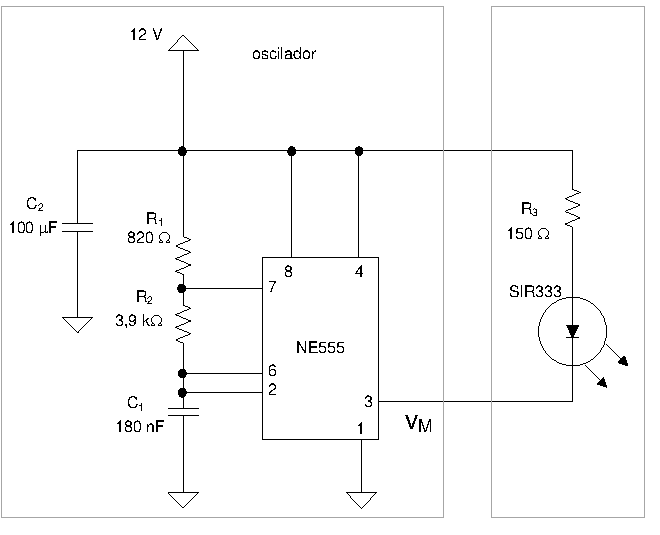
\includegraphics{Imagens/emissor.pdf}
    \caption{Circuito representativo do emissor de IV.}
    \label{fig:emissor}
\end{figure}

\subsubsection{Análise teórica}

Em primeiro lugar analisa-se o circuito da Fig. \ref{fig:emissor}. Destaca-se o papel do condensador $C_2$ como condensador de contorno, pois para altas frequências funciona como um curto-circuito, eliminando o ruído de $V_{CC}$. As resistências $R_1$ e $R_2$ e o condensador $C_1$ são necessários para o normal funcionamento do temporizador NE555 como será explicado posteriormente. O propósito da resistência $R_3$ é limitar a corrente que atravessa o díodo SIR333.

O funcionamento do circuito emissor pode ser dividido em 3 fases. Na primeira, que é iniciada pela ligação à alimentação, tem-se que o condensador $C_1$ é carregado por $V_{CC}$ através de $R_1$ e $R_2$, pelo que a sua tensão evolui em resposta a um degrau. Simultaneamente, a tensão no condensador, $V_{C_1}$, está a ser comparada com $\frac{1}{3} V_{CC}$ no comparador ligado à porta 2 do NE555 (cujo circuito interno está representado na Fig. \ref{fig:timer}) e com $\frac{2}{3} V_{CC}$ no comparador ligado à porta 6 do NE555. Assim, enquanto o condensador carrega desde $0 \si{\volt}$ até $\frac{1}{3} V_{CC}$, é aplicado ao \textit{flip-flop} $\textit{Set} = 1$ devido ao comparador ligado à porta 2 do NE555 e $\textit{Reset} = 0$ devido ao comparador ligado à porta 6 do NE555, pelo que a saída do \textit{flip-flop}, $V_M$, é $V_{OH}$. Quando $\frac{1}{3} V_{CC} < V_{C_1} < \frac{2}{3} V_{CC}$, tem-se $\textit{Set} = 0$ e $\textit{Reset} = 0$, pelo que o estado do \textit{flip-flop} não se altera. Como o flip-flop está a \textit{High}, o transístor está ao corte e, portanto, não há descarregamento do condensador $C_1$ através dele. Termina, assim, a fase 1.

\begin{figure}[ht]
    \centering
    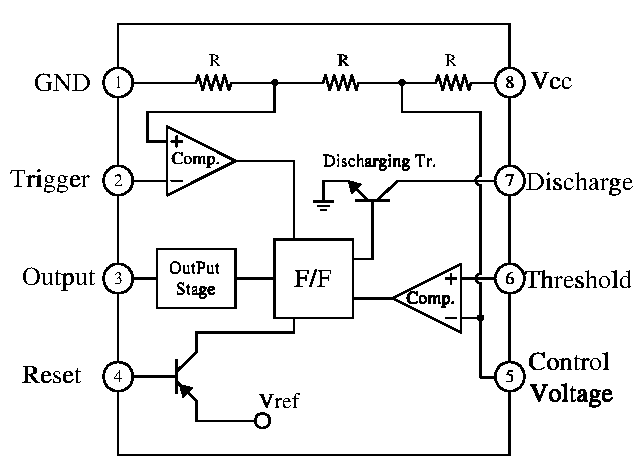
\includegraphics{Imagens/ne555_circuito.pdf}
    \caption{Circuito representativo do NE555 Single Timer.}
    \label{fig:timer}
\end{figure}

Quando, instantaneamente, a tensão no condensador ultrapassa $\frac{2}{3} V_{CC}$, tem-se $\textit{Set} = 0$ e $\textit{Reset} = 1$, pelo que o estado do \textit{flip-flop} passa a \textit{Low}, o transístor deixa de estar ao corte e o condensador $C_1$ descarrega através dele e da resistência $R_2$. A fase 2 estabelece-se, então, para $\frac{1}{3} V_{CC} < V_{C_1} < \frac{2}{3} V_{CC}$ com descarregamento do condensador $C_1$.

A tensão no condensador $C_1$ ultrapassará agora instantaneamente $\frac{1}{3} V_{CC}$, pelo que $\textit{Set} = 1$ e $\textit{Reset} = 0$, o estado do \textit{flip-flop} passa a \textit{High}, o transístor passa a estar ao corte novamente e o condensador $C_1$ carrega como anteriormente. A fase 3 estabelece-se, então, para $\frac{1}{3} V_{CC} < V_{C_1} < \frac{2}{3} V_{CC}$ com carregamento do condensador $C_1$. Assim, em estado estacionário existe uma alternância entre as fases 2 e 3. De acordo com o apresentado anteriomente e no manual do NE555 Single Timer, pode-se escrever
\begin{align}
    V_{C_1} (t) &= \left\{
\begin{array}{ll}
\left (1- e^{-\frac{t}{(R_1+R_2) C_1}} \right) V_{CC} &, \; \text{fase 1} \\
\frac{2}{3} e^{-\frac{t}{\left (R_2 + R_D \right) C_1}} V_{CC} &, \; \text{fase 2} \\
\left (1-\frac{2}{3} e^{-\frac{t}{(R_1+R_2) C_1}} \right) V_{CC} &, \; \text{fase 3}
\end{array}\; \text{e}
\right. \label{VC1}\\
V_M (t) &= \left\{
\begin{array}{ll}
V_{OH} \quad, \; \text{fases 1 e 3} \\
V_{OL} \quad, \; \text{fase 2}
\end{array}\;,
\right. \label{VM}
\end{align}
obtendo-se as formas de onda obtidas representadas na Fig. \ref{fig:VM_VC1_tempo}.

\begin{figure}[ht]
    \centering
    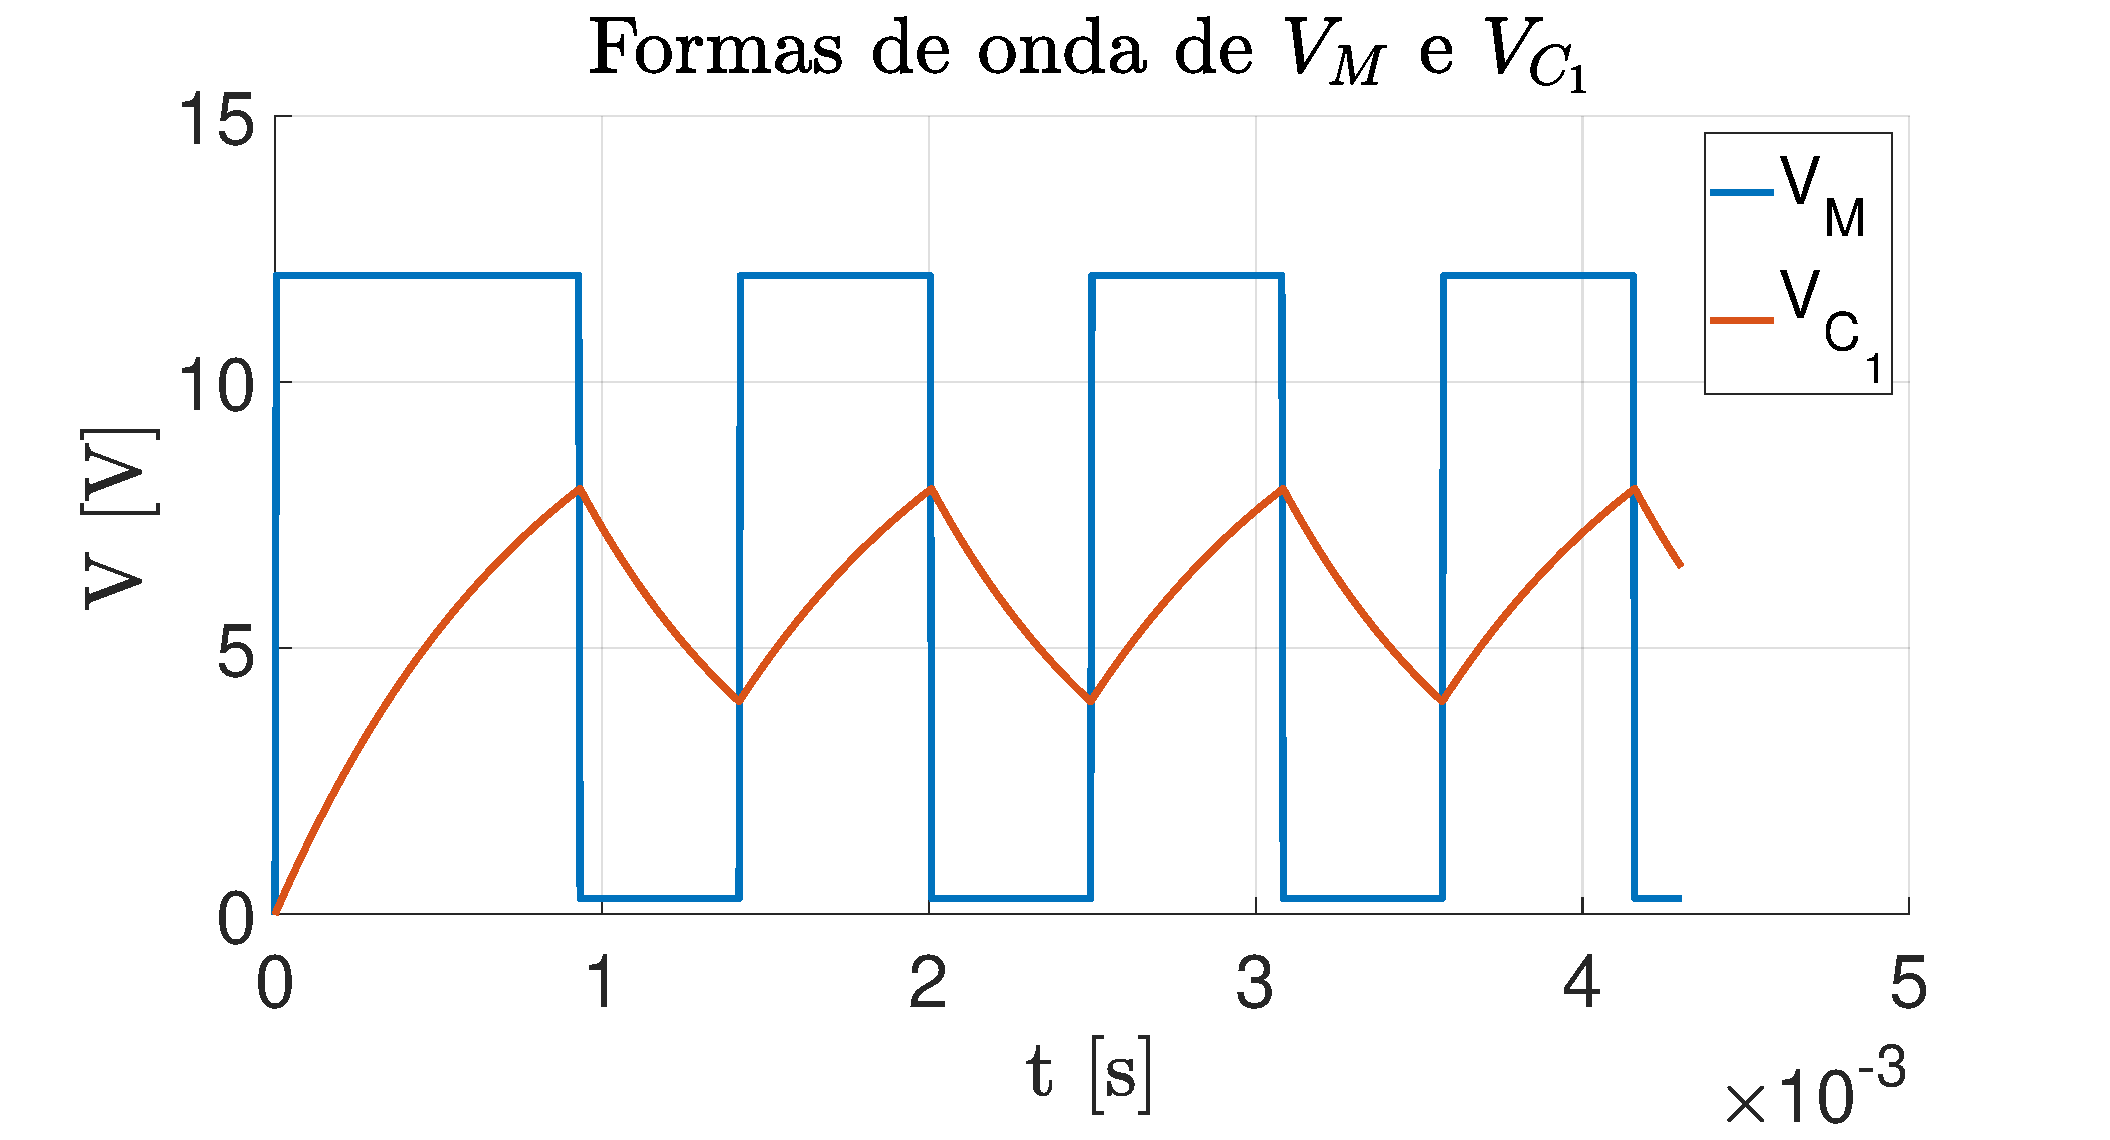
\includegraphics[width=\linewidth]{Imagens/VM_VC1_tempo.pdf}
    \caption{Formas de onda de $V_{C_1}$ e $V_M$.}
    \label{fig:VM_VC1_tempo}
\end{figure}

$V_{OH}$ é aproximado por $V_{CC}$ e $V_{OL}$ pelo valor indicado no manual para $V_{CC} = 15 \si{\volt}$ e $I_{SINK} = 50 \si{\milli \ampere}$, ou seja, $V_{OL} = 0,3 \si{\volt}$. Os tempos de descarga e de carga obtidos das expressões anteriores, i.e., os tempos das fases 2 e 3, respetivamente, (também apresentados no manual) são
\begin{align}
    T_L &= \ln (2) C_1 R_2 \quad \text{e} \label{eq:T_L_expressao} \\
    T_H &= \ln (2) C_1 (R_1 + R_2) \label{eq:T_H_expressao}\:.
\end{align}
A partir de \eqref{eq:T_H_expressao} e \eqref{eq:T_L_expressao}, escreve-se
\begin{align}
    f &= \frac{1}{T} = \frac{1}{\ln(2) C_1 (R_1 + 2 R_2)} \approx 930 \si{\hertz} \quad \text{e}\\
    \text{fator de ciclo} &=\frac{T_H}{T_H + T_L} = \frac{R_1+R_2}{R_1+2 R_2} \approx 0.548 \label{eq:fatordeciclo}
\end{align}

Para descobrir a corrente máxima, aplica-se a lei das malhas ao circuito do emissor (Fig. \ref{fig:emissor}) e faz-se 
\begin{equation}
    V_{CC} - V_M + R_3 i + V_{SIR} (i) \label{i_max_condicao}\:,
\end{equation}
onde $V_{SIR}$ é a tensão no díodo. Quando se maximiza a corrente, maximiza-se $V_{CC} - V_M$, pelo que deve utilizar-se a mínima tensão de saída do oscilador, ou seja, $V_{OL}$, para obter a corrente máxima.

Surgem, então, dois métodos de resolução. No primeiro, afirma-se que a tensão do díodo quando está em condução é constante e, tendo em conta o valor dado pelo manual para $I = 100 \si{\milli \ampere}$ ($I$ corresponde à corrente no díodo), igual a $1.4 \si{\volt}$, resultando em
\begin{equation*}
    i_{max} = \frac{V_{CC} - V_{OL} - 1.4}{R_3} \approx 68.7 \si{\milli \ampere}\:.
\end{equation*}

No segundo método, utiliza-se a caraterística tensão-corrente do díodo dada pelo manual para $T = 25 \si{\celsius}$. Após a aplicação de um método iterativo, observa-se que $i_{max} \approx 70 \si{\milli \ampere}$ respeita a caraterística do díodo e a condição imposta por \eqref{i_max_condicao}. Ambos os métodos apresentam soluções idênticas como seria de esperar e ambas se encontram abaixo da corrente máxima que o díodo suporta a $\SI{25}{\celsius}$, $i_{maxOp}=\SI{100}{\milli\ampere}$.

Por outro lado, o valor mínimo de $R_3$ é também obtido a partir de \eqref{i_max_condicao} com $V_M$ mínima, pois $R_3$ tem de permitir ao circuito o funcionamento tanto em \textit{High} como em \textit{Low}, mas agora com $i_{maxOp}$. Para $i = i_{maxOp} = 100 \si{\milli \ampere}$, $V_{SIR} = 1.4 \si{\volt}$ de acordo com o manual, pelo que se obtém
\begin{equation*}
    R_{3_{\mathrm{min}}} = \frac{V_{CC} - V_{OL} - 1.4}{0.100} \approx 103 \si{\ohm}\:.
\end{equation*}




\subsubsection{Trabalho experimental}
\vspace{2mm}
\noindent\textbf{3.1.2.1 \hspace{1mm}Formas de Onda} \par
Depois de feita a montagem, representada na Fig. \ref{fig:emissor}, foi possível observar no osciloscópio o gráfico representado na Fig. \ref{fig:formas_onda}, em que a forma de onda de $V_{C_1}$ está representada a verde e a forma de onda de $V_M$ está representada a laranja.
\begin{figure}[ht]
    \centering
    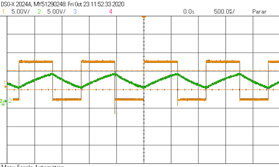
\includegraphics[width=8cm]{Imagens/oscilador_formas_onda.png}
    \caption{Formas de onda de $V_{C_1}$ (verde) e $V_M$(laranja)}
    \label{fig:formas_onda}
\end{figure}

Foram medidos os valores do período dos ciclos \textit{High} e o período do ciclo total, já que só são necessários estes dois parâmetros para calcular o fator de ciclo e a frequência de oscilação. Estas medidas foram feitas no osciloscópio, tendo-se pondo um marcador no início do período que se estava a medir e outro no final, devolvendo o osciloscópio a diferença de tempo entre estes dois pontos, isto é, o período.  O fator de ciclo é calculado usando \eqref{eq:fatordeciclo}. As medições realizadas estão representados na Tabela \ref{tab:períodos_tabela}, tanto para $V_M$ como para $V_{C_1}$, assim como o fator de ciclo e a frequência de oscilação ($f=\frac{1}{T}$) que foram calculados posteriormente. 
\begin{table}[ht]
    \centering
    \caption{Período, fator de ciclo e frequência para cada sinal.}
    \begin{tabular}{ccccc}
    \hline
         Sinal & $T [ms]$ & $T_{H} [ms]$ & fator de ciclo & $f [Hz]$\\
        \hline
        $V_M$   & 1.14 & 0.610 &    0.535 & 877\\
         $V_{C_1}$   & 1.14 & 0.620 &  0.544  & 877\\
    \hline
    \end{tabular}
    \label{tab:períodos_tabela}
\end{table}

\vspace{2mm}
\noindent\textbf{3.1.2.2 \hspace{1mm}Corrente no Díodo} \par
Para o cálculo do díodo primeiramente foi feita a medição do $V_{cc}=11.32 V$. Posteriormente foi feita a medição entre o terminal do $R_3$ comum ao díodo e a massa, apresentada a azul na Fig. \ref{fig:diodi}. O seu valor mínimo toma $V^{\mathrm{min}}_{R_3/GND}=1.83V$. Podemos assim facilmente calcular a tensão que percorre $R_3$ através da diferença entre estas duas tensões e consequentemente calcular a corrente no díodo, como pedido.
\begin{equation}
\label{eq:tensao_r3}
    V_{R_3}= V_{cc} -V^{\mathrm{min}}_{R_3/GND} =  11.32 - 1.83 = 9.49 V
\end{equation}
A corrente que passa no díodo é facilmente calculada através da Lei de Ohm, sabendo o valor de $V_{R_3}$ calculado em (\ref{eq:tensao_r3}) e o valor da resistência $R_3=148.6 \ohm$, podemos escrever
\begin{equation*}
    \frac{V_{R3}}{R_3} = I_3 = 63.9 mA \: .
\end{equation*}



\begin{figure}
    \centering
    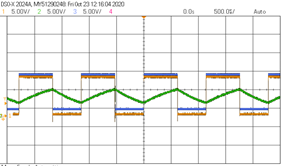
\includegraphics[width = 0.55\textwidth]{Imagens/diodo.png}
    \caption{Formas de Onda: $V_{C_1}$ a verde, $V_M$ a laranja, saída de R3 a azul. }
    \label{fig:diodi}
\end{figure}


\subsubsection{Comparação de Resultados}
Procedemos então agora à comparação entre os resultados teóricos e os resultados experimentais obtidos. A Tabela \ref{tab:resultados_oscilador} resume a informação obtida.

\begin{table}[h!]
    \centering
    \caption{Valores teóricos e experimentais de $R_3$, $i_3$, fator de ciclo, e $f$.}
    \begin{tabular}{cccc}
    \hline
    Parâmetro & Valor experimental & Valor teórico & Erro relativo (\%) \\
    \hline  
    $f_{V_m}$ [Hz]  & 877  & 930  & -5.70 \\
    fator de ciclo ($V_M$) & 0.535  & 0.548 & -2.37 \\
    $f_{V_{C1}}$ [Hz]  & 877  & 930  & -5.70 \\
    fator de ciclo ($V_{C_1}$) & 0.544  & 0.548  & -0.730\\\
    $i_3$ [mA] & 63.9  & 68.7  & -6.99 \\
    \hline
    \end{tabular}
    \label{tab:resultados_oscilador}
\end{table}
Em primeiro lugar, esperava-se que o valor da frequência fosse igual tanto para onda $V_M$ como para a onda $V_{C_1}$ o que de facto se verificou, tendo ambas o valor de 877 Hz. Em relação ao valor teórico registou-se um erro relativo de -5.70 \%, este erro pode ser explicado pelas grandes tolerâncias associados ao valor da capacidade dos condensadores. 

Em segundo lugar, podemos analisar os valores do fator de ciclo. Aqui, também esperávamos que tanto para $V_M$ como para $V_{C_1}$ o valor fosse igual entre os dois. Isto não se verificou, mas a diferença entre os dois valores é bastante pequena, sendo que o valor do fator de ciclo $V_M$ apenas se encontra deslocado de cerca de -1.65 \% em relação ao valor do fator de ciclo $V_{C_1}$. As diferenças entre o valor experimental e o valor teórico são bastante inferiores às verificadas para a frequência. Na verdade, o fator de ciclo depende apenas dos valores das resistências, que têm uma tolerância significativamente mais pequena que as dos condensadores, pelo que seria de esperar que o erro verificado fosse mais pequeno. 

Em terceiro lugar, analisando a corrente do díodo, o erro associado em relação ao valor teórico é de -6.99\% . Uma das razões para este erro ser ligeiramente maior do que seria desejável está relacionado com as assumpções que foram feitas para o cálculo do valor teórico. Uma vez que a \textit{datasheet} só apresenta valores para $V_{cc}= 15 V$ estes valores tiveram que ser utilizados apesar de  o valor de $V_{cc}$ com que trabalhámos tenha sido 12 V. Adicionalmente, existe ainda uma componente de erro associada ao valor de $V_{cc}$. Os cálculos teóricos foram realizados com $V_{cc}= 12V$, mas confirmámos que durante a experiência o valor de $V_{cc}$ que foi de facto utilizado foi 11.32 V, o que representa um erro de cerca de -5.67\% . 

%Finalmente, é ainda de salientar que alguns dos erros podem também estar associados aos componentes eletrónicos utilizados. Estes componentes têm sempre uma tolerância a si associados e portanto os valores utilizados para os cálculos teóricos raramente são iguais aos valores efetivamente presentes no circuito.
%Comparando com os valores teóricos, em ambos os casos se obtiveram erros relativos baixos, sendo o valor do erro de $V_{C_1}$ ligeiramente menor que o valor do erro de $V_M$, estando um erro de -0.730 \% associado ao primeiro e um erro de -2.37 \% associado ao segundo. 
% Porém, apesar de as assumpções que tiveram de ser feitas, consideramos que os resultados experimentais foram bons comparados com os resultados teóricos. Para finalizar a resistência $R_3$ mínima calculada foi de 103 \ohm, tendo a resistência $R_3$ o valor de 148.6 \ohm, sendo portanto maior que a resistência mínima como esperado.\par